\documentclass{scrbook}
\usepackage{graphicx} % Required for inserting images
\usepackage{tabularx} % Required for fixed width tables
\usepackage{scrlayer-scrpage} % Required for the subtitles
\usepackage{url} % Required for the URLs
\usepackage{hyperref} % Required for the URLs
\usepackage{listings} % Required for the code snippets
\usepackage{mathtools} % Required for the system of equations
\usepackage{enumitem} % Required for list styling

\usepackage{fontspec}
\setmonofont{DejaVu Sans Mono} % Overleaf has this font pre-installed

% Put the caption of the snippets at the bottom
\lstset{
	captionpos=b,
	basicstyle=\ttfamily\small,
	columns=fullflexible,
	keepspaces=true
}


\title{DNS: Domain Name Service}
\subtitle{Ambient intelligence course (A.Y. 2025/2026)\\Topic taught by Prof. Floriano Scioscia}
\author{Gabriele Colapinto}
\date{\today}

\begin{document}
	
	\maketitle
	\thispagestyle{empty}
	
	{\Large\textbf{License}} \\
	{Notes from Ambient intelligence (A.Y. 2025/2026) by Gabriele Colapinto. 
		Course taught by professors Michele Ruta, Floriano Scioscia, Arnaldo Tomasino, Davide Loconte — 
		Licensed under CC BY-NC 4.0.\\
		\url{https://creativecommons.org/licenses/by-nc/4.0/}}
	
	\vspace*{\fill}
	\rule{\textwidth}{0.2pt}
	\small{© 2025 Gabriele Colapinto \\
		Released under the \href{https://creativecommons.org/licenses/by-nc/4.0/}{Creative Commons Attribution–NonCommercial 4.0 International License}}
	
	\clearpage
	
	\tableofcontents

	\chapter{DNS Foundations: Namespace, Delegation, and Resolution}
	
	\section{Purpose of the Domain Name System}
	
	The Domain Name System (DNS) is the naming infrastructure that relates logical names to numerical network addresses. Its most visible function is the translation of hostnames into IP addresses, for example:
	\begin{itemize}
	    \item \texttt{sisinflab.poliba.it} $\rightarrow$ \texttt{193.204.49.75};
	    \item \texttt{www.google.it} $\rightarrow$ \texttt{66.233.183.104}.
	\end{itemize}
	Hostnames are suitable for users and applications because they are mnemonic and independent from the numerical representation used by the network layer. IP addresses, instead, are the identifiers used for forwarding packets. DNS reconciles these two requirements by providing a distributed directory service.\\
	
	DNS is not limited to direct name-to-address translation. It also supports reverse mappings from IP addresses to hostnames and special-purpose records, such as mail exchange records used to locate the mail servers responsible for a domain. For instance, when a mail address such as \texttt{f.scioscia@poliba.it} is processed, the part after \texttt{@} is used to query the DNS for mail exchange information associated with \texttt{poliba.it}.\\
	
	The system has three complementary components:
	\begin{itemize}
	    \item a hierarchical naming scheme based on domains;
	    \item a distributed database implementing that hierarchy;
	    \item a protocol used by clients, resolvers, and name servers to query, maintain, and distribute the corresponding records.
	\end{itemize}
	The protocol is used both between a client and a DNS server and among DNS servers during the resolution process. From the point of view of an application, DNS appears as a translation service invoked before contacting the destination host. Internally, however, the answer may require interaction with several servers in different parts of the DNS hierarchy.
	
	\section{Hierarchical Namespace}
	
	\begin{figure}
		\centering
		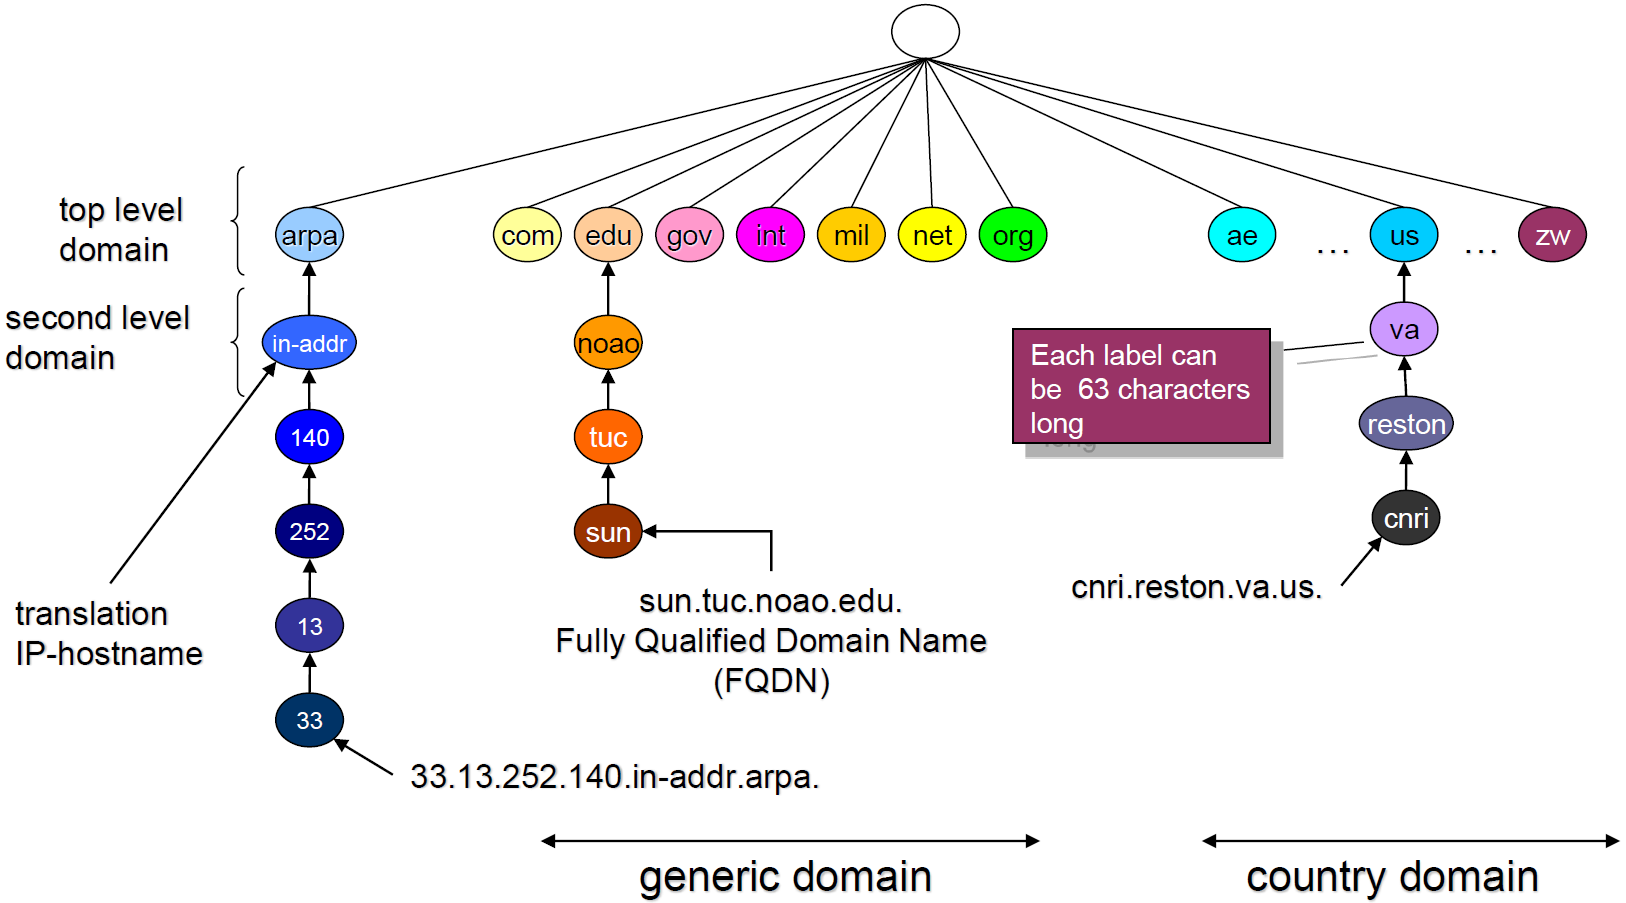
\includegraphics[width=\linewidth]{Images/DNS_namespace.png}
		\caption{DNS hierarchical namespace}
		\label{fig:dns_namespace}
	\end{figure}
	
	The DNS namespace is organized as an inverted tree (see figure \ref{fig:dns_namespace}). The root is the highest level and is conventionally represented by the empty label, often written as a final dot. Below the root there are top-level domains, including generic top-level domains such as \texttt{com}, \texttt{edu}, \texttt{gov}, \texttt{int}, \texttt{mil}, \texttt{net}, and \texttt{org}, and country-code top-level domains such as \texttt{it}, \texttt{ae}, \texttt{us}, and \texttt{zw}. Lower levels identify organizations, subdomains, and individual hosts.\\
	
	A domain is a subtree of the namespace. A domain can contain hosts and further subdomains; therefore, administrative control can be delegated progressively along the tree. A fully qualified domain name (FQDN) identifies an object by specifying its complete path in the DNS hierarchy, ending at the root. Examples are:
	\begin{itemize}
	    \item \texttt{sun.tuc.noao.edu.};
	    \item \texttt{cnri.reston.va.us.};
	    \item \texttt{33.13.252.140.in-addr.arpa.}.
	\end{itemize}
	The final dot denotes that the name is absolute with respect to the root. Each label in a DNS name can be at most 63 characters long.\\
	
	The branch \texttt{in-addr.arpa} is used for reverse IPv4 lookups. It represents IP address components as DNS labels in reverse order. Thus, the address \texttt{140.252.13.33} corresponds to the DNS name \texttt{33.13.252.140.in-addr.arpa.}. This construction allows reverse mapping to reuse the same hierarchical DNS machinery used for ordinary names.
	
	\section{Zones, Delegation, and Authority}
	
	A zone is the portion of the DNS namespace administered by a specific authority. The boundary of a zone does not necessarily coincide with the boundary of a domain: an organization may manage an entire domain directly, or it may delegate some subdomains to other administrative entities.\\
	
	Top-level domains are administered by registries. For country-code top-level domains, such as \texttt{it}, the registry function is associated with the national Network Information Center and follows the corresponding ISO country-code allocation. For lower zones, management is delegated to organizations that are responsible for the correctness and availability of the records in their part of the namespace.\\
	
	For each zone there is a primary authoritative name server and one or more secondary name servers. The primary server manages the authoritative copy of the zone data. Secondary servers maintain replicated copies for redundancy and availability, updating their data from the primary server according to configured synchronization policies. This replication is essential because name resolution must remain available even when a server fails or becomes temporarily unreachable.\\
	
	An authoritative server directly manages the mappings for its zone. When it answers for a name contained in that zone, the response is authoritative: the server is not merely reporting cached information obtained elsewhere, but is providing data from the administrative source responsible for that zone.\\
	
	At the top of the namespace there are the root name servers (see figure \ref{fig:dns_root_servers}). The root corresponds to the domain ``\texttt{.}'' and provides the starting point for discovering the servers responsible for top-level domains. In the traditional DNS model there are thirteen root name server identities. Operationally, these identities can be replicated through distributed deployments, but the logical role is the same: they provide delegation information for top-level domains, not ordinary host records for the entire Internet.\\
	
	The root is therefore a bootstrap point for the hierarchy. Knowing that a name ends in \texttt{.it} or \texttt{.com} is not sufficient to know which name servers are authoritative for that top-level domain. A resolver must obtain that delegation information, and the root zone is the stable place from which this discovery begins when the relevant information is not already cached.
	
	\begin{figure}
		\centering
		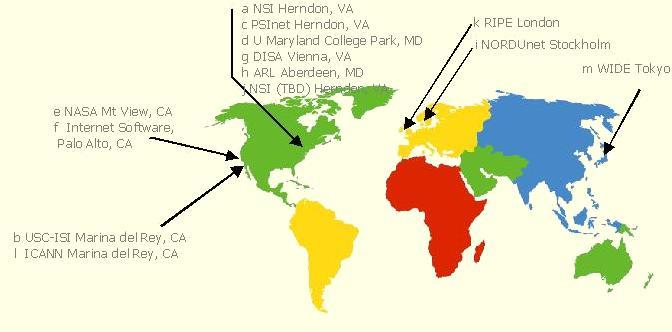
\includegraphics[width=\linewidth]{Images/DNS_root_servers.jpg}
		\caption{DNS root name servers}
		\label{fig:dns_root_servers}
	\end{figure}
	
	\section{Name Resolution}
	
	\begin{figure}
		\centering
		\includegraphics[width=0.5\linewidth]{Images/recursive_DNS_call.png}
		\caption{Example of recursive DNS call}
		\label{fig:recursive_dns_call}
	\end{figure}
	
	Name resolution is the process that transforms a requested DNS name into the required record data. Consider a host \texttt{host1.poliba.it} that needs the IP address of \texttt{host2.mydomain.eu} (see figure \ref{fig:recursive_dns_call}). The host normally does not traverse the DNS hierarchy directly. It sends the query to its configured local DNS server, for example \texttt{dns.poliba.it}. The local server acts as a resolver and obtains the answer on behalf of the client.\\
	
	With an empty cache, the resolution path can be represented as follows:
	\begin{lstlisting}
host1.poliba.it
  -> dns.poliba.it
  -> root name server
  -> .eu top-level-domain name server
  -> dns.mydomain.eu
  <- address record for host2.mydomain.eu
	\end{lstlisting}
	The root server does not normally return the final address of \texttt{host2.mydomain.eu}. Instead, it returns the name servers responsible for \texttt{eu}. The \texttt{eu} top-level-domain server then returns the authoritative name servers for \texttt{mydomain.eu}. Finally, the authoritative server for \texttt{mydomain.eu}, such as \texttt{dns.mydomain.eu}, returns the record for \texttt{host2.mydomain.eu}.\\
	
	Publicly reachable hosts are normally served through at least two authoritative name servers, so that the availability of the name does not depend on a single server. The DNS hierarchy is therefore both administrative and operational: delegation assigns responsibility, while replication and caching improve availability and performance.
	
	\subsection{Recursive Resolution}
	
	In recursive resolution, the client delegates the entire lookup to a recursive resolver. The client sends a query and expects either the final answer or an error. The resolver performs the necessary steps through the DNS hierarchy, follows delegations, queries authoritative servers, and returns the result to the client.\\
	
	This mode is preferable from the viewpoint of an ordinary end host because it minimizes the number of DNS exchanges performed by the client. The computational and network burden is moved to the recursive resolver, which is usually operated by an Internet service provider, an organization, a campus network, a public DNS provider, or a local network device.\\
	
	A recursive resolver still needs an initial point from which to discover the hierarchy. This bootstrap information is typically provided by a small and stable configuration known as root hints, containing root server names and addresses. The resolver can then refresh its knowledge of the root server set through the DNS protocol itself.
	
	\subsection{Iterative Resolution}
	
	\begin{figure}[!h]
		\centering
		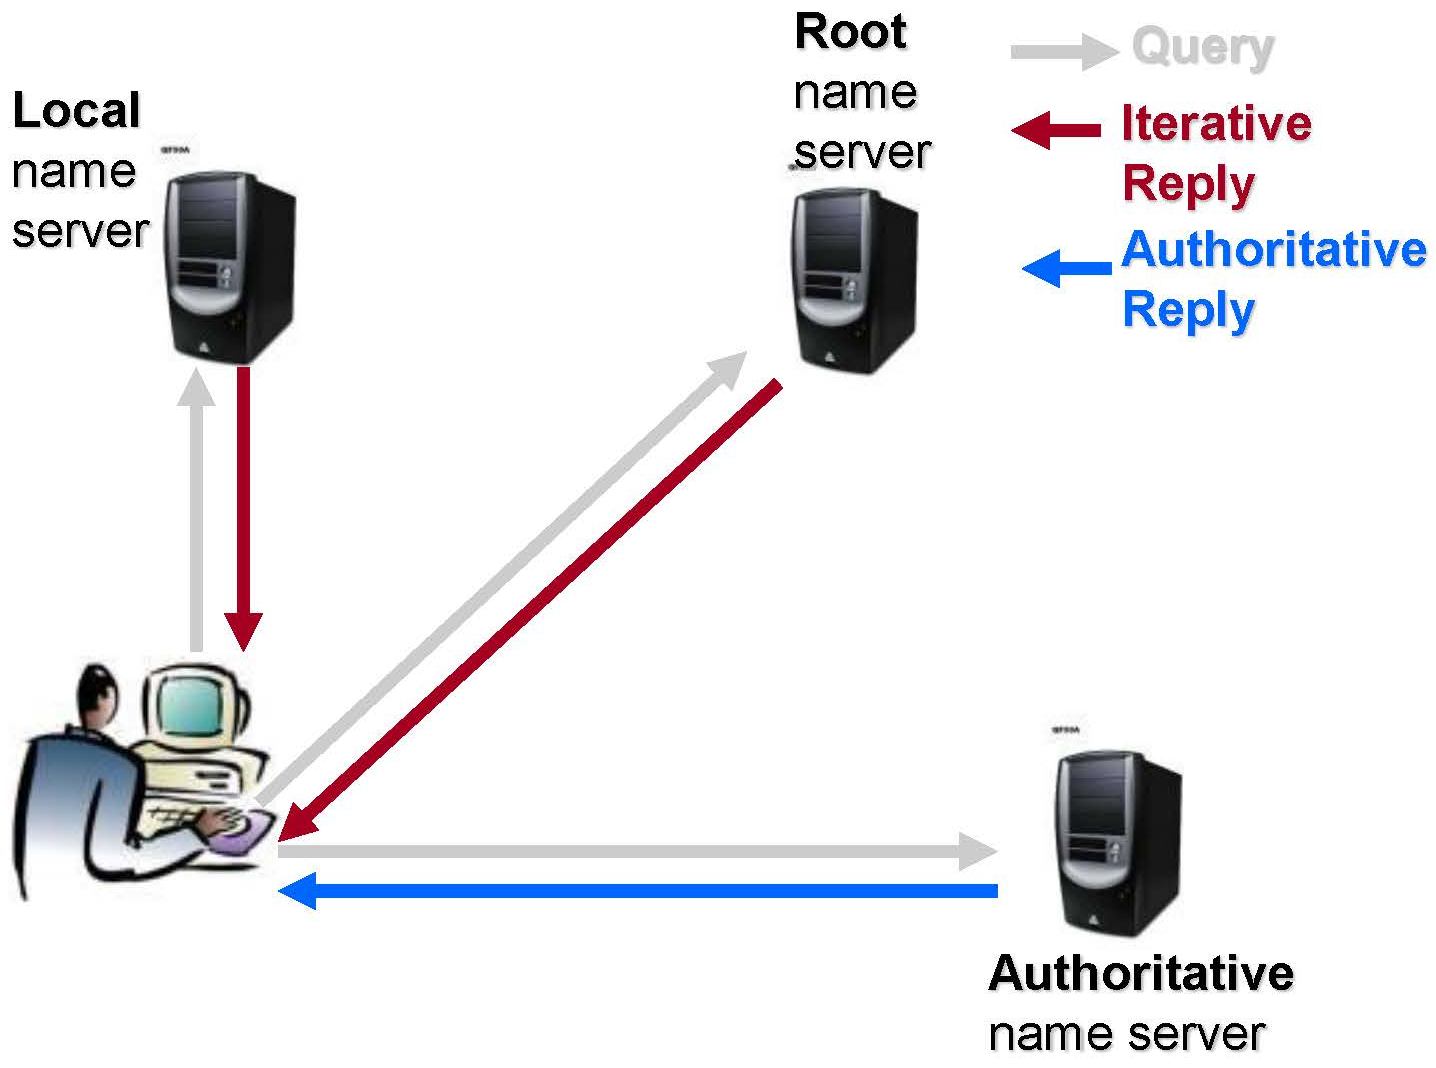
\includegraphics[width=0.5\linewidth]{Images/Iterative_address_resolution.png}
		\caption{Example of iterative DNS call}
		\label{fig:iterative_dns_call}
	\end{figure}
	
	In iterative resolution, a server that does not know the final answer returns the best referral it can provide. The requester is then responsible for querying the next server. The process continues until an authoritative answer is obtained or the lookup fails.\\
	
	Iterative resolution shifts work toward the requester. If an ordinary client used it directly, the client would generate more DNS traffic and maintain more resolution state. It would also need to process referrals and choose the next servers to contact. For this reason, recursive resolution is normally preferred at the client side.\\
	
	The iterative model can nevertheless reduce delay in some situations, especially when the resolver already has useful cached delegations and can contact the appropriate authoritative server without repeating the full path from the root. In practice, recursive resolvers commonly use iterative queries when communicating with the DNS hierarchy, while end hosts use recursive service offered by their configured resolver.
	
	\section{Caching and Non-authoritative Answers}
	
	\begin{figure}[!h]
		\centering
		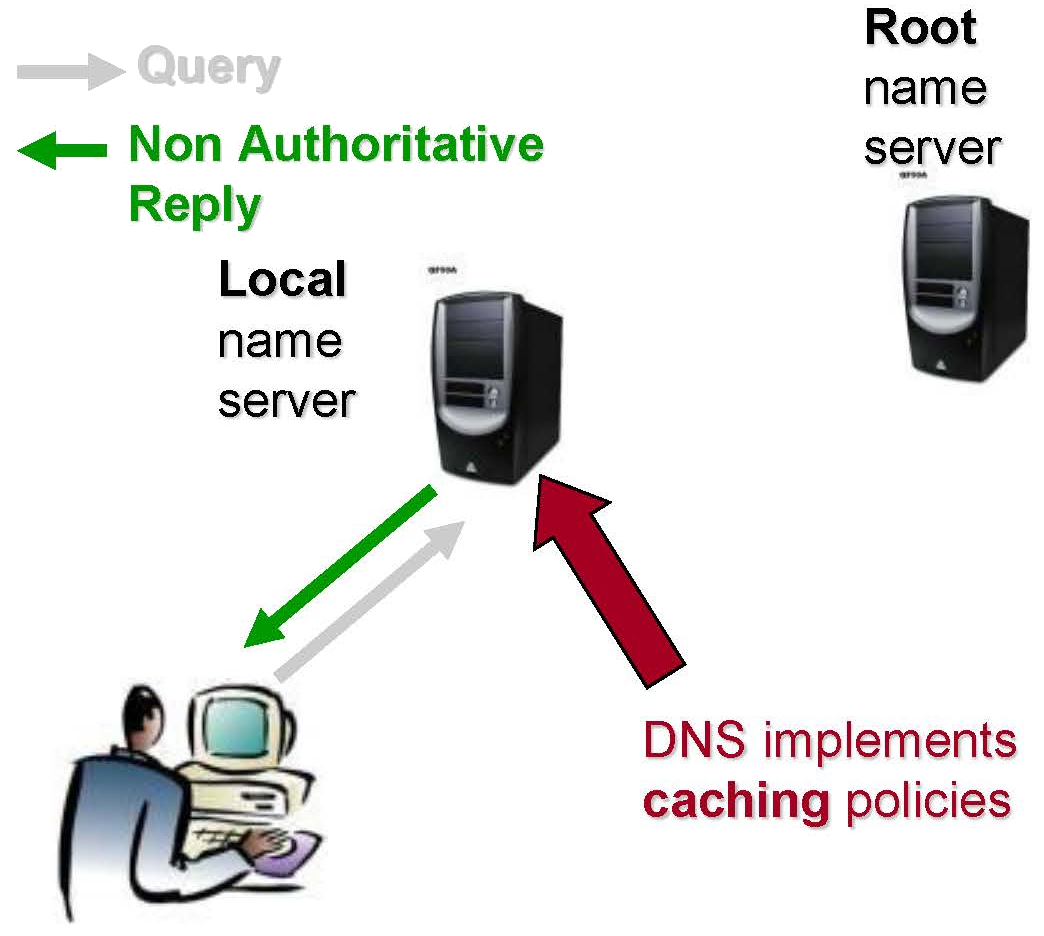
\includegraphics[width=0.5\linewidth]{Images/Non_authoritative_answer.png}
		\caption{The user queries the local name server and it returns a non authoritative answer using its cached data.}
		\label{fig:non_authoritative_answer}
	\end{figure}
	
	DNS implements caching to reduce resolution delay and network traffic. When a local name server receives a response, it may store the returned records and reuse them for later queries. If another client asks for the same name before the cached data expires, the local server can answer immediately without querying the hierarchy again.\\
	
	Caching is especially effective because many clients in the same administrative network tend to access the same services. It also reduces load on root, top-level-domain, and authoritative servers. The performance benefit, however, introduces a distinction between authoritative and non-authoritative answers.\\
	
	A non-authoritative answer is a response generated from cached data by a server that is not authoritative for the queried zone. Such an answer may be operationally useful and perfectly valid, but it is not the original administrative source of the data. Cached records are associated with a finite lifetime, after which they must be considered stale and removed or refreshed.\\
	
	The distinction matters for correctness and security. DNS data can change over time, and cached data may temporarily reflect an older state. Moreover, cache alteration attacks can attempt to inject fraudulent mappings into a resolver cache. For this reason, diagnostic tools and protocol fields explicitly expose whether an answer is authoritative. Later protocol extensions also allow resolvers to signal whether data has been authenticated according to their validation policies.\\
	
	Caching therefore improves scalability and latency, but it must be interpreted together with authority, lifetime, and validation information. A fast answer is not necessarily an authoritative one; a correct resolver must preserve this distinction when returning and reporting DNS results.
	
	\chapter{DNS Message Format and Resource Records}
	
	\section{DNS Messages as Transactions}
	
	\begin{figure}[!h]
		\centering
		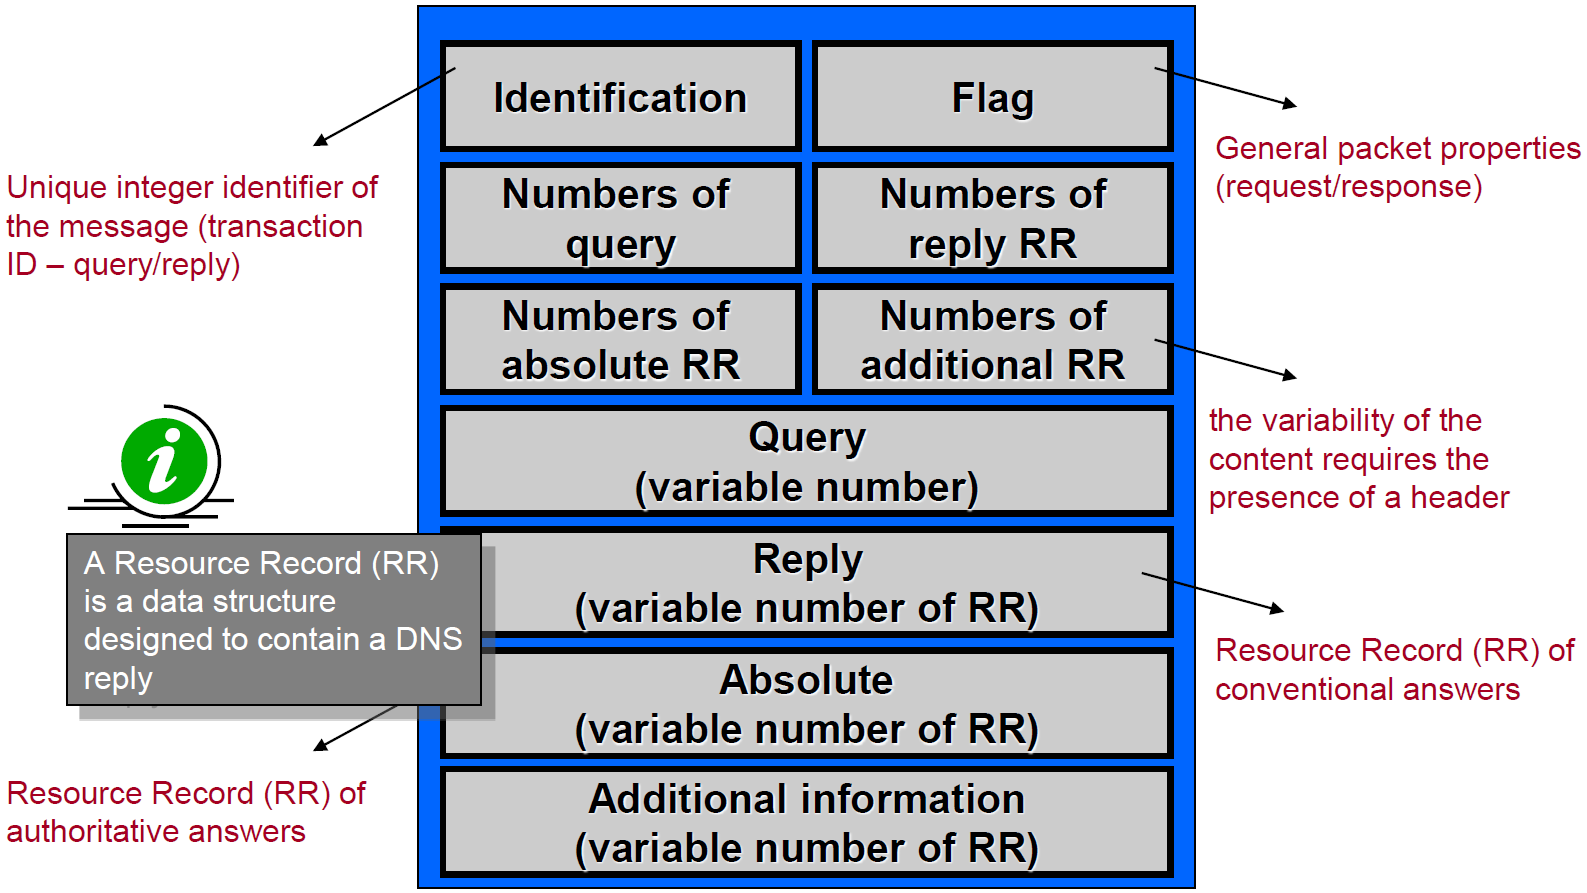
\includegraphics[width=0.5\linewidth]{Images/DNS_message.png}
		\caption{Structure of a DNS message}
		\label{fig:dns_message_structure}
	\end{figure}
	
	DNS communication is based on request--response messages. A client or resolver sends a query containing the name and type of information it wants to obtain; the server replies with a message that carries the same transaction identifier and, when available, the requested records. Since DNS commonly operates over UDP, the transaction identifier is essential to associate each response with the corresponding query without relying on a persistent transport connection.\\
	
	A DNS message has a fixed-size header followed by a variable number of records (see figure \ref{fig:dns_message_structure}). The header specifies the properties of the message and the number of elements contained in each subsequent section:
	\begin{itemize}
	    \item the \textbf{question section}, containing the query or queries;
	    \item the \textbf{answer section}, containing resource records that directly answer the query;
	    \item the \textbf{authority section}, containing records related to authoritative name servers;
	    \item the \textbf{additional section}, containing auxiliary records useful to complete the interpretation of the answer or to continue the resolution process.
	\end{itemize}
	
	The first field, \texttt{Identification}, is a 16-bit integer chosen by the requester. The same value is copied into the response, allowing the requester to match the reply with the query. The next 16 bits form the flag field, which encodes the type of message, the requested resolution mode, and the outcome of the operation. The following four counters indicate how many entries are present in the question, answer, authority, and additional sections. These counters are necessary because the last four sections have variable size.\\
	
	A DNS response may contain more information than the single record requested by the client. For example, a query for an address record may return a chain of canonical-name records, one or more final address records, the name servers responsible for the relevant domain, and additional address records for those name servers. This structure allows DNS to return not only a result, but also information that can reduce the cost of subsequent resolutions.
	
	\section{The Flag Field}
	
	The flag field is a compact 16-bit structure:
	\begin{center}
		\begin{tabular}{|c|c|c|c|c|c|c|c|c|c|c|}
			\hline
			
			\textbf{Fields} & QR & opcode & AA & TC & RD & RA & Z & AD & CD & rcode \\ \hline
			
			\textbf{Bits} & 1 & 4 & 1 & 1 & 1 & 1 & 1 & 1 & 1 & 4 \\ \hline
		\end{tabular}
	\end{center}
	
	Each subfield has a specific role in describing the message or the response status.
	
	\subsection{Message Type and Operation}
	
	The \texttt{QR} bit distinguishes queries from responses. A value of \texttt{0} marks a query, while \texttt{1} marks a response. The \texttt{opcode} field identifies the kind of operation requested:
	\begin{itemize}
	    \item \texttt{0}: standard query, typically used to map a name to the requested record type;
	    \item \texttt{1}: reverse query, historically associated with address-to-name lookup;
	    \item \texttt{2}: server status request;
	    \item \texttt{3}: reserved;
	    \item \texttt{4}: notify, used to signal changes to a zone;
	    \item \texttt{5}: update, used for dynamic DNS updates;
	    \item \texttt{6--15}: reserved.
	\end{itemize}
	
	The dominant case in ordinary resolution is the standard query. The specific meaning of the query is then determined by the resource record type, such as \texttt{A}, \texttt{PTR}, \texttt{CNAME}, \texttt{NS}, or \texttt{MX}.
	
	\subsection{Authority, Truncation, and Recursion}
	
	The \texttt{AA} bit, meaning \emph{Authoritative Answer}, is meaningful in responses. It is set to \texttt{1} when the responding server is authoritative for the queried name. If it is \texttt{0}, the answer may still be usable, but it is not guaranteed directly by the zone authority; it may have been obtained from a cache.\\
	
	The \texttt{TC} bit indicates truncation. In the basic UDP-based DNS message format, a response that exceeds the maximum supported size may be truncated. A truncated answer signals that the requester cannot assume that the received message contains the complete response.\\
	
	The \texttt{RD} bit, meaning \emph{Recursion Desired}, is set by the requester. When \texttt{RD=1}, the requester asks the server to perform recursive resolution on its behalf. When \texttt{RD=0}, the requester does not ask for recursion and can follow referrals iteratively.\\
	
	The \texttt{RA} bit, meaning \emph{Recursion Available}, is set by the server in responses. It indicates whether the server supports recursive resolution. Thus, \texttt{RD} expresses what the client wants, while \texttt{RA} expresses what the server is able or willing to provide.
	
	\subsection{Reserved and Validation-Related Bits}
	
	The \texttt{Z} bit is reserved and is normally set to \texttt{0}. The \texttt{AD} bit, meaning \emph{Authenticated Data}, indicates that the server considers the answer authenticated according to its validation policies. The \texttt{CD} bit, meaning \emph{Checking Disabled}, indicates that checking of the data has been disabled for the query.\\
	
	These bits are relevant when DNS data validation is used. In the basic interpretation of a query or response, they are still part of the packet and must be parsed correctly even when no validation decision is being made by the local application.
	
	\subsection{Return Codes}
	
	The final four bits form the \texttt{rcode} field. It is used in responses to report the result of the operation:
	\begin{itemize}
	    \item \texttt{0}: no error;
	    \item \texttt{1}: format error;
	    \item \texttt{2}: server failure;
	    \item \texttt{3}: name error;
	    \item \texttt{4}: not implemented;
	    \item \texttt{5}: refused;
	    \item \texttt{6}: \texttt{YXDomain}, a name exists when it should not;
	    \item \texttt{7}: \texttt{YXRRSet}, a resource record set exists when it should not;
	    \item \texttt{8}: \texttt{NXRRSet}, a resource record set that should exist does not;
	    \item \texttt{9}: \texttt{NotAuth}, the server is not authoritative for the zone;
	    \item \texttt{10}: \texttt{NotZone}, the name is not contained in the zone;
	    \item \texttt{11--15}: reserved.
	\end{itemize}
	
	The return code must be interpreted together with the other fields. For instance, a response with \texttt{rcode=0} and \texttt{AA=0} is successful but non-authoritative, while a response with \texttt{rcode=9} indicates that the contacted server is not authoritative for the relevant zone.
	
	\newpage
	\section{Resource Record Format}
	
	A Resource Record (RR) is the basic data unit used by DNS to represent one piece of information about a name. A record may express, for example, an address mapping, an alias, a delegation to a name server, a mail exchanger, or a reverse mapping. In DNS messages, a Resource Record has the following general wire format:
	\begin{lstlisting}
 0                   15 16                  31
+----------------------+----------------------+
| Domain name                                 |
| variable length, encoded as DNS labels      |
+----------------------+----------------------+
| Type                 | Class                |
| 16 bits              | 16 bits              |
+----------------------+----------------------+
| Time-to-live                                |
| 32 bits                                     |
+----------------------+----------------------+
| Data length          | Data                 |
| 16 bits              | variable length      |
+----------------------+----------------------+
	\end{lstlisting}
	
	The \texttt{domain name} field, also called \texttt{NAME}, identifies the DNS name to which the record applies. Its length is variable because DNS names are encoded as sequences of labels rather than as fixed-size strings. Each label is preceded by its length, and the name is terminated by a zero-length label. DNS name compression may also be used inside messages.\\
	
	The \texttt{type} field is 16 bits long and defines the semantics of the record. In the cases considered here, type \texttt{1} denotes an \texttt{A} record, used for name-to-IPv4-address translation, while type \texttt{12} denotes a \texttt{PTR} record, used for reverse address-to-name translation through the \texttt{in-addr.arpa} namespace. Other record types, such as \texttt{CNAME}, \texttt{NS}, and \texttt{MX}, extend DNS beyond direct host address lookup.\\
	
	The \texttt{class} field is 16 bits long and identifies the protocol family or record class. For ordinary Internet DNS data, the class is \texttt{IN}, numerically represented as \texttt{1}.\\
	
	The \texttt{time-to-live} field is 32 bits long and specifies, in seconds, how long the record may remain in a resolver cache before it must be considered expired. A resolver that reuses a cached record must decrement the effective remaining lifetime and discard the record when the TTL reaches zero.\\
	
	The \texttt{data length} field, also called \texttt{RDLENGTH}, is 16 bits long and gives the size in bytes of the following \texttt{data} field. The \texttt{data} field, also called \texttt{RDATA}, has variable length because its structure depends on the record type. For an \texttt{A} record, \texttt{RDATA} contains a 32-bit IPv4 address. For a \texttt{PTR} record, it contains a domain name used as the target of a reverse mapping. For a \texttt{CNAME} record, it contains the canonical name associated with an alias. For an \texttt{NS} record, it contains the hostname of an authoritative name server.
	
	\subsection{Main DNS Resource Record Types}
	
	The \texttt{type} field determines how the \texttt{RDATA} field of a Resource Record must be interpreted. DNS defines many record types, not all of which are commonly used in ordinary name resolution. For the purposes of understanding DNS operation, it is useful to distinguish the main functional categories of records: address records, aliasing records, delegation records, mail records, text and policy records, reverse-resolution records, DNSSEC records, and service-discovery records.
	
	\begin{table}[!h]
		\centering
		\begin{tabular}{lll}
			\hline
			\textbf{Type} & \textbf{Code} & \textbf{Purpose} \\
			\hline
			\texttt{A} & \texttt{1} & Maps a domain name to an IPv4 address. \\
			\texttt{AAAA} & \texttt{28} & Maps a domain name to an IPv6 address. \\
			\texttt{CNAME} & \texttt{5} & Defines an alias for a canonical domain name. \\
			\texttt{NS} & \texttt{2} & Identifies an authoritative name server for a zone. \\
			\texttt{SOA} & \texttt{6} & Provides administrative information about a zone. \\
			\texttt{PTR} & \texttt{12} & Maps a reverse DNS name to a domain name. \\
			\texttt{MX} & \texttt{15} & Identifies mail exchangers for a domain. \\
			\texttt{TXT} & \texttt{16} & Stores textual data, often used for domain policies. \\
			\texttt{SRV} & \texttt{33} & Locates services by protocol, domain, port, and priority. \\
			\texttt{CAA} & \texttt{257} & Specifies which certificate authorities may issue certificates. \\
			\hline
		\end{tabular}
		\caption{Common DNS Resource Record types.}
	\end{table}
	
	The \texttt{A} and \texttt{AAAA} records are address records. They are the standard mechanism for associating a hostname with an IP address. An \texttt{A} record contains a 32-bit IPv4 address, whereas an \texttt{AAAA} record contains a 128-bit IPv6 address. These records are the most direct form of name-to-address translation.\\
	
	The \texttt{CNAME} record defines an alias. Its \texttt{RDATA} field does not contain an IP address, but another domain name, called the canonical name. Resolution therefore continues by querying the canonical name. A \texttt{CNAME} is useful when several names must refer to the same service endpoint, but the actual address records should be maintained under only one canonical name.\\
	
	The \texttt{NS} and \texttt{SOA} records describe zone authority. An \texttt{NS} record identifies a name server authoritative for a domain or zone. An \texttt{SOA} record marks the start of a zone and contains administrative parameters such as the primary name server, the responsible mailbox, the zone serial number, and timing values used by secondary servers for synchronization.\\
	
	The \texttt{PTR} record is used for reverse resolution. Instead of mapping a hostname to an address, it maps a specially constructed name in the reverse namespace, such as \texttt{in-addr.arpa} for IPv4, to a hostname. This record type is commonly used when an application or administrator needs to determine the symbolic name associated with an IP address.\\
	
	The \texttt{MX} record supports mail routing. It associates a domain with one or more mail exchangers, each with a preference value. Mail transfer agents use these records to select the host to which incoming mail for a domain should be delivered.\\
	
	The \texttt{TXT} record stores text associated with a domain name. Although originally general-purpose, it is widely used to publish machine-readable domain policies, such as sender authorization and domain ownership verification data.\\
	
	The \texttt{SRV} record generalizes service location. Instead of only resolving a hostname to an address, it allows a domain to publish the hostname and port number of a service, together with priority and weight values. This is useful for protocols that need to discover service endpoints dynamically.\\
	
	The \texttt{CAA} record is used in the certificate issuance process. It allows a domain owner to specify which certificate authorities are authorized to issue certificates for that domain, reducing the risk of unauthorized certificate issuance.\\
	
	Several additional record types are used by DNSSEC. The most important are summarized in Table~\ref{tab:dnssec-record-types}.
	
	\begin{table}[!h]
		\centering
		\begin{tabular}{lll}
			\hline
			\textbf{Type} & \textbf{Code} & \textbf{Purpose} \\
			\hline
			\texttt{DNSKEY} & \texttt{48} & Publishes a DNSSEC public key for a zone. \\
			\texttt{DS} & \texttt{43} & Links a delegated zone to a parent-zone trust chain. \\
			\texttt{RRSIG} & \texttt{46} & Stores a digital signature over an RRset. \\
			\texttt{NSEC} & \texttt{47} & Authenticated denial of existence. \\
			\texttt{NSEC3} & \texttt{50} & Hashed authenticated denial of existence. \\
			\hline
		\end{tabular}
		\caption{Main DNSSEC-related Resource Record types.}
		\label{tab:dnssec-record-types}
	\end{table}
	
	DNSSEC records do not replace ordinary DNS records. Instead, they add authentication data that allows a validating resolver to verify that the received data is consistent with the signed DNS hierarchy. For example, an \texttt{A} record still contains the IPv4 address of a host, while the corresponding \texttt{RRSIG} record contains the signature needed to validate that address record as part of an RRset.\\
	
	Some record types are special-purpose, obsolete, experimental, or rarely used. Examples include \texttt{HINFO}, historically used to describe host information; \texttt{CERT}, used to store certificates; \texttt{TLSA}, used by DANE to associate TLS information with a name; and \texttt{SVCB} and \texttt{HTTPS}, which provide service binding information for modern connection establishment. These records illustrate that DNS is not only a hostname-to-address database, but a general distributed naming infrastructure whose record semantics are extensible through the \texttt{type} field.
	
	\newpage
	\section{A Standard Type \texttt{A} Query}
	
	A type \texttt{A} query requests the IPv4 address associated with a domain name. In a typical client-to-local-resolver exchange, the client sends a DNS query to the configured DNS server on port \texttt{53}. The following trace summarizes the relevant fields of a query for \texttt{www.google.it}:
	\begin{lstlisting}
DNS Standard query A www.google.it

Flags: 0x0100
QR      = 0  message is a query
opcode  = 0  standard query
TC      = 0  message is not truncated
RD      = 1  recursion desired
Z       = 0  reserved bit unset
AD/CD   = 0  no authenticated-data decision in the query

Questions:      1
Answer RRs:     0
Authority RRs:  0
Additional RRs: 0

Question:
Name:  www.google.it
Type:  A
Class: IN
	\end{lstlisting}
	
	The query contains one question and no answer, authority, or additional records. The \texttt{QR} bit marks the message as a query. The \texttt{opcode} indicates a standard query. The \texttt{RD} bit is set, meaning that the client asks the contacted server to perform recursive resolution if the answer is not already known.\\
	
	The absence of answer records is expected: the query only declares what information is being requested. The name \texttt{www.google.it}, the type \texttt{A}, and the class \texttt{IN} fully specify the question from the resolver's point of view.
	
	\section{A Standard Type \texttt{A} Response}
	
	A successful response may include a richer set of records than the final IPv4 addresses. The following response to the previous query contains a canonical-name chain, two address records, authority information, and additional address records:
	\begin{lstlisting}
DNS Standard query response

Flags: 0x8180
QR      = 1  message is a response
opcode  = 0  standard query
AA      = 0  server is not authoritative for the domain
TC      = 0  message is not truncated
RD      = 1  recursion was requested
RA      = 1  recursion is available
Z       = 0  reserved bit unset
AD      = 0  answer was not authenticated by the server
rcode   = 0  no error

Questions:      1
Answer RRs:     4
Authority RRs:  4
Additional RRs: 4
	\end{lstlisting}
	
	The response is successful because \texttt{rcode=0}. It is non-authoritative because \texttt{AA=0}: the server that returned the response is not the authority for the queried domain. It may have obtained the result by recursion or from its cache. The pair \texttt{RD=1} and \texttt{RA=1} indicates that recursion was requested and that the server supports recursive queries.
	
	\subsection{Answer Section}
	
	The answer section may contain records of different types when aliases are involved:
	\begin{lstlisting}
Answers:

www.google.it: type CNAME, class IN, TTL 3d1h1m19s, cname www.google.com
www.google.com: type CNAME, class IN, TTL 8m18s, cname www.l.google.com
www.l.google.com: type A, class IN, TTL 23s, addr 66.249.85.104
www.l.google.com: type A, class IN, TTL 23s, addr 66.249.85.99
	\end{lstlisting}
	
	The first two records are \texttt{CNAME} records. They do not directly provide an IP address; instead, they identify canonical names that must be followed until an address-bearing record is reached. In this case, \texttt{www.google.it} is resolved through \texttt{www.google.com} and then through \texttt{www.l.google.com}. The final two \texttt{A} records provide IPv4 addresses for \texttt{www.l.google.com}.\\
	
	Multiple \texttt{A} records for the same name are common. They allow a domain to associate a logical service name with several network endpoints. DNS can then return the set of addresses, often with ordering policies that contribute to load distribution and fault tolerance. The time-to-live values associated with these records determine how long resolvers may reuse the mappings without asking again.
	
	\subsection{Authority and Additional Sections}
	
	The authority section identifies name servers that are authoritative for the relevant domain:
	\begin{lstlisting}
Authority nameservers:

l.google.com: type NS, class IN, ns b.l.google.com
l.google.com: type NS, class IN, ns c.l.google.com
l.google.com: type NS, class IN, ns d.l.google.com
l.google.com: type NS, class IN, ns a.l.google.com
	\end{lstlisting}
	
	Each \texttt{NS} record states that the domain \texttt{l.google.com} is served by one of the listed authoritative name servers. These records are useful both for the current resolution and for future queries concerning the same portion of the namespace.\\
	
	The additional section can provide address records for the name servers listed in the authority section:
	\begin{lstlisting}
Additional records:

b.l.google.com: type A, class IN, addr 64.233.179.9
c.l.google.com: type A, class IN, addr 64.233.161.9
d.l.google.com: type A, class IN, addr 64.233.183.9
a.l.google.com: type A, class IN, addr 216.239.53.9
	\end{lstlisting}
	
	These additional \texttt{A} records avoid extra lookups for the addresses of the authoritative name servers. Without them, a resolver that receives the \texttt{NS} names may still need to resolve those names before it can contact the corresponding servers. The additional section therefore reduces latency and network traffic by carrying useful auxiliary information together with the main answer.
	
	\section{Authoritative and Non-Authoritative Answers}
	
	The distinction between authoritative and non-authoritative answers is central to correct DNS interpretation. An authoritative answer is returned by a server that directly manages the zone containing the queried name. A non-authoritative answer is returned by a server that is not the zone authority, typically because it has cached the result or has obtained it through recursive resolution.\\
	
	Non-authoritative answers are not inherently wrong. They are essential to the scalability of DNS because caches reduce both resolution delay and query load on authoritative servers. However, they must be constrained by time-to-live values and interpreted with awareness of cache freshness. A resolver may use a cached answer until its TTL expires; after that, it must refresh the information before using it again.\\
	
	The \texttt{AA} flag provides the protocol-level indication of authority. In a response with \texttt{AA=1}, the responding server is authoritative for the queried domain. In a response with \texttt{AA=0}, the record may still be valid, but the response is not a direct statement from the authority for that zone. This distinction is particularly important when diagnosing incorrect mappings, cache inconsistency, or suspected cache manipulation.
	
	\chapter{Reverse Resolution and Mail Exchange Records}
	
	\section{Specialized DNS Queries}
	
	DNS is commonly introduced through direct name-to-address resolution, but the same infrastructure also supports queries whose purpose is not simply to obtain an address for a hostname. Two relevant cases are reverse resolution and mail exchange discovery.\\
	
	Reverse resolution starts from an IP address and asks for the corresponding domain name. It is implemented through \texttt{PTR} records and a dedicated portion of the DNS namespace. Mail exchange discovery starts from a mail domain and asks which hosts are responsible for accepting mail for that domain. It is implemented through \texttt{MX} records and is used by mail transfer agents when routing e-mail.\\
	
	Both mechanisms preserve the same basic DNS message structure introduced earlier: a query specifies a name, a type, and a class; a response contains one or more resource records, possibly with authority and additional sections. What changes is the interpretation of the queried name and of the returned data.
	
	\section{Reverse Resolution with \texttt{PTR} Records}
	
	\subsection{Purpose of Reverse DNS}
	
	A \texttt{PTR} (pointer) query is used when the requester knows an IP address and wants to obtain the hostname associated with that address. This operation is the inverse of a direct \texttt{A} query at the conceptual level, but it is not performed by searching the DNS database backwards. DNS remains a name-indexed hierarchy, so an IP address must first be converted into a domain name placed under a reverse-resolution subtree.\\
	
	Reverse DNS is useful in diagnostics, logging, network administration, and policy checks. For example, a server log may contain an IP address and a diagnostic tool may perform a reverse lookup to display a more meaningful hostname. The result, however, should not be interpreted as a proof of identity: it is a DNS record controlled by the authority responsible for the corresponding address space.
	
	\subsection{The \texttt{in-addr.arpa} Namespace}
	
	For IPv4 addresses, reverse mappings are placed under the \texttt{in-addr.arpa} domain. The address octets are written in reverse order because DNS names are hierarchical from right to left, while IPv4 routing prefixes are naturally read from left to right. Reversing the octets aligns DNS delegation with IP address delegation.\\
	
	For example, the IPv4 address
	\begin{lstlisting}
140.252.13.33
	\end{lstlisting}
	is represented in the reverse DNS namespace as:
	\begin{lstlisting}
33.13.252.140.in-addr.arpa.
	\end{lstlisting}
	
	The rightmost part, \texttt{in-addr.arpa}, identifies the reverse IPv4 namespace. The label \texttt{140} corresponds to the first octet of the address, then \texttt{252}, then \texttt{13}, and finally \texttt{33}. This order allows the namespace to delegate authority consistently with address blocks. An organization responsible for a prefix can manage the corresponding subtree and publish \texttt{PTR} records for addresses inside that block.\\
	
	A reverse lookup therefore does not ask directly for ``the name of an IP address''. It asks for a \texttt{PTR} record whose owner name is the reversed representation of that address in the reverse DNS tree.
	
	\subsection{Structure of a \texttt{PTR} Query}
	
	A reverse query for an IPv4 address is a standard DNS query whose type is \texttt{PTR}. For instance, to resolve \texttt{193.204.59.227} into a hostname, the queried name is:
	\begin{lstlisting}
227.59.204.193.in-addr.arpa
	\end{lstlisting}
	
	The DNS question is therefore:
	\begin{lstlisting}
Name:  227.59.204.193.in-addr.arpa
Type:  PTR
Class: IN
	\end{lstlisting}
	
	At the packet level, the request has the same general properties as a standard query. A typical query contains one question, no answer records, no authority records, and no additional records:
	\begin{lstlisting}
DNS Standard query PTR 227.59.204.193.in-addr.arpa

Transaction ID: 0x0004

Flags: 0x0100
QR      = 0  message is a query
opcode  = 0  standard query
TC      = 0  message is not truncated
RD      = 1  recursion desired
Z       = 0  reserved bit unset
AD/CD   = 0  no authenticated-data decision in the query

Questions:      1
Answer RRs:     0
Authority RRs:  0
Additional RRs: 0
	\end{lstlisting}
	
	The \texttt{opcode} remains the standard query opcode. The fact that this is a reverse lookup is expressed by the queried name and by the \texttt{PTR} type, not by using a different message structure. The \texttt{RD} flag may be set when the client wants the contacted resolver to perform recursive resolution.
	
	\subsection{\texttt{PTR} Response}
	
	A successful \texttt{PTR} response contains a resource record whose data field is a domain name. For the previous example, the answer may be summarized as:
	\begin{lstlisting}
227.59.204.193.in-addr.arpa   PTR   dee227.poliba.it
	\end{lstlisting}
	
	The response header may indicate that the answer is authoritative:
	\begin{lstlisting}
DNS Standard query response PTR dee227.poliba.it

Flags: 0x8580
QR      = 1  message is a response
opcode  = 0  standard query
AA      = 1  server is authoritative for the domain
TC      = 0  message is not truncated
RD      = 1  recursion was requested
RA      = 1  recursion is available
Z       = 0  reserved bit unset
AD      = 0  answer was not authenticated by the server
rcode   = 0  no error

Questions:      1
Answer RRs:     1
Authority RRs:  4
Additional RRs: 4
	\end{lstlisting}
	
	The \texttt{AA=1} flag indicates that the responding server is authoritative for the reverse zone containing the queried name. The answer section contains one \texttt{PTR} record:
	\begin{lstlisting}
Name:         227.59.204.193.in-addr.arpa
Type:         PTR
Class:        IN
Time to live: 12 hours
Data length: 18
Domain name:  dee227.poliba.it
	\end{lstlisting}
	
	The time-to-live determines how long this reverse mapping can be cached. As with other DNS records, a cached \texttt{PTR} answer is reusable only until its TTL expires.
	
	\newpage
	\subsection{Authority and Additional Records in Reverse Lookup}
	
	A reverse lookup response may also include authority records for the reverse zone. For example:
	\begin{lstlisting}
Authority nameservers:

59.204.193.in-addr.arpa: type NS, class IN, ns cstar.poliba.it
59.204.193.in-addr.arpa: type NS, class IN, ns server2.garr.net
59.204.193.in-addr.arpa: type NS, class IN, ns anthares.poliba.it
59.204.193.in-addr.arpa: type NS, class IN, ns dns2.nic.it
	\end{lstlisting}
	
	These records state which name servers are authoritative for the reverse zone. They are structurally analogous to the authority records returned in direct resolution, but the zone is part of \texttt{in-addr.arpa} rather than a conventional organizational domain.\\
	
	The additional section may provide address records for those name servers:
	\begin{lstlisting}
Additional records:

cstar.poliba.it: type A, class IN, addr 193.204.49.36
server2.garr.net: type A, class IN, addr 131.154.1.11
anthares.poliba.it: type A, class IN, addr 193.204.49.37
dns2.nic.it: type A, class IN, addr 193.205.245.8
	\end{lstlisting}
	
	These additional records make the response more useful to a resolver, because they avoid extra address lookups for the authoritative name servers listed in the authority section.
	
	\subsection{Using Command-Line Tools for Reverse Lookup}
	
	A reverse lookup can be requested with tools that construct the \texttt{PTR} query automatically from the IP address. For example:
	\begin{lstlisting}
host 193.204.59.227
	\end{lstlisting}
	
	A possible result is:
	\begin{lstlisting}
227.59.204.193.in-addr.arpa domain name pointer dee227.poliba.it.
	\end{lstlisting}
	
	The tool hides the construction of the reverse name, but the DNS query still targets\\
	\texttt{227.59.204.193.in-addr.arpa} with type \texttt{PTR}. This is useful for interactive diagnostics, while packet-level analysis remains necessary when the goal is to inspect flags, authority information, or caching behavior.
	
	\newpage
	\section{Mail Exchange Resolution with \texttt{MX} Records}
	
	\subsection{Role of \texttt{MX} Records}
	
	When an e-mail message is sent through the Internet, the sender's Mail Transfer Agent (MTA) must determine which server can accept incoming mail for the recipient's domain. The domain is the part of the address after the \texttt{@} symbol. For an address such as:
	\begin{lstlisting}
f.scioscia@poliba.it
	\end{lstlisting}
	the relevant mail domain is:
	\begin{lstlisting}
poliba.it
	\end{lstlisting}
	
	The MTA performs a DNS query of type \texttt{MX} for that domain. The response returns one or more mail exchange records. Each record identifies a mail server hostname and associates it with a preference value. The MTA uses these records to decide where to deliver the message.
	
	\subsection{Preference Values and Server Selection}
	
	An \texttt{MX} response may contain multiple mail exchangers for the same domain. Each exchanger is associated with a numeric preference. Lower values indicate higher preference, so the sender should try the mail server with the lowest preference value first.\\
	
	Conceptually, an \texttt{MX} answer has the following form:
	\begin{lstlisting}
domain.example.   MX   10 mail1.domain.example.
domain.example.   MX   20 mail2.domain.example.
domain.example.   MX   30 mail3.domain.example.
	\end{lstlisting}
	
	In this example, \texttt{mail1.domain.example} is tried before \texttt{mail2.domain.example}, because \texttt{10} is lower than \texttt{20}. If delivery to the preferred server fails, the MTA can try the next available exchanger according to the preference order. This mechanism supports redundancy and controlled failover for mail delivery.\\
	
	When several records have the same preference value, the sender may distribute attempts among them. This allows a domain to use several mail servers at the same priority level, combining availability with load distribution.
	
	\subsection{\texttt{MX} Records and Mail Server Address Resolution}
	
	An \texttt{MX} record specifies which host is responsible for receiving e-mail for a domain. The value returned by an \texttt{MX} query is not an IP address, but the hostname of a \emph{mail exchanger}. A mail exchanger is therefore the DNS name of a host that can accept incoming mail on behalf of the queried domain.\\
	
	For example, the domain \texttt{example.org} may have an \texttt{MX} record pointing to \texttt{mail.example.net}. In this case, \texttt{example.org} is the domain used in the recipient's e-mail address, while \texttt{mail.example.net} is the host that receives mail for that domain. Before opening an SMTP connection, the Mail Transfer Agent (MTA) must resolve \texttt{mail.example.net} to an IP address, usually by issuing an \texttt{A} query for IPv4 or an \texttt{AAAA} query for IPv6.\\
	
	The complete logical sequence is therefore:
	\begin{enumerate}
		\item extract the recipient domain from the e-mail address;
		\item query DNS for the \texttt{MX} records of that domain;
		\item select the mail exchanger according to the preference value;
		\item resolve the selected mail exchanger hostname through an \texttt{A} or \texttt{AAAA} query;
		\item open an SMTP connection to the resulting IP address.
	\end{enumerate}
	
	The distinction between the domain and the mail exchanger is important. The domain is the logical destination used in e-mail addresses, such as \texttt{user@example.org}. The mail exchanger is the actual DNS host designated to receive mail for that domain, such as \texttt{mail.example.net}. This indirection allows a domain to change its mail infrastructure by updating its \texttt{MX} records, without changing users' e-mail addresses. It also allows the same domain to publish multiple mail exchangers for redundancy and load distribution.
	
	\subsection{Multiple Mail Servers for a Domain}
	
	The \texttt{MX} mechanism provides a clean way to associate a single mail domain with several mail servers. This is different from merely returning multiple address records for one name: \texttt{MX} records express service-specific routing information. They state which hosts are responsible for a service, not just which addresses correspond to a name.\\
	
	For example, a domain may publish one primary mail exchanger and one backup exchanger. The backup server may have a higher preference value and receive messages only when the primary server is unavailable. Alternatively, a domain may publish several exchangers with equal preference to distribute delivery attempts among them.\\
	
	The DNS answer may also include additional address records for the listed mail exchangers, when available. These records reduce the number of subsequent lookups required by the sender. However, the authoritative information for mail routing remains the \texttt{MX} record itself: the associated address records are only the next step needed to contact the selected host.
	
	\section{Comparison Between \texttt{A}, \texttt{PTR}, and \texttt{MX} Queries}
	
	The three query types considered so far illustrate different uses of the same DNS infrastructure:
	\begin{itemize}
	    \item \texttt{A} records map a hostname to an IPv4 address;
	    \item \texttt{PTR} records map a reverse DNS name to a hostname;
	    \item \texttt{MX} records map a mail domain to one or more mail exchanger hostnames with preference values.
	\end{itemize}
	
	The queried name and the record type determine the semantics of the response. In an \texttt{A} query, the name is the service or host name whose address is required. In a \texttt{PTR} query, the name is a reversed representation of an IP address under \texttt{in-addr.arpa}. In an \texttt{MX} query, the name is a mail domain, and the returned data identifies hosts responsible for mail reception.\\
	
	These differences also affect how applications use the result. A web client usually needs an address record before opening a connection to a server. A diagnostic tool may use a \texttt{PTR} record to display the hostname associated with an address. A mail transfer agent uses \texttt{MX} records to choose the next SMTP destination and then performs address resolution for that destination.
	
	\section{Operational Considerations}
	
	Reverse and mail exchange records depend on correct delegation and maintenance of the corresponding zones. A valid direct \texttt{A} record does not imply the existence of a corresponding \texttt{PTR} record, and a \texttt{PTR} record does not guarantee that the returned hostname resolves back to the same address. Forward and reverse DNS are related operationally, but they are represented by distinct records, often managed in different zones.\\
	
	Similarly, the existence of a domain name does not imply that the domain is configured to receive mail. Mail reception requires suitable \texttt{MX} records, or an equivalent fallback behavior depending on the mail system and standards in use. In operational configurations, explicit \texttt{MX} records are preferred because they clearly identify the hosts responsible for the mail service and allow multiple servers with ordered preferences.\\
	
	Caching applies to both \texttt{PTR} and \texttt{MX} records. Their TTL values influence how quickly changes in reverse mappings or mail routing become visible to resolvers and sending systems. Shorter TTLs allow faster changes but increase DNS query load; longer TTLs reduce load but delay propagation of configuration changes. For mail services, this trade-off is particularly relevant during migrations, when exchangers and preference values may need to change without interrupting delivery.
	
	\chapter{DNS Diagnostic Tools and Query Inspection}
	
	\section{Role of Diagnostic Tools in DNS Analysis}
	
	DNS diagnostic tools provide a practical interface to the resolution mechanisms and record types introduced in the previous chapters. They are useful for verifying name-to-address mappings, checking reverse mappings, inspecting mail exchange configuration, identifying authoritative servers, and distinguishing authoritative answers from cached non-authoritative answers.\\
	
	The tools considered here operate at different levels of detail:
	\begin{itemize}
	    \item \texttt{nslookup} provides a simple interactive or command-line interface for common DNS queries;
	    \item \texttt{host} offers compact output for direct, reverse, and selected record-type queries;
	    \item \texttt{dig} exposes the structure of DNS replies in a form close to the protocol message format;
	    \item \texttt{whois} queries registration databases at registry level and is therefore complementary to DNS resolution.
	\end{itemize}
	
	Although these tools can query similar records, they are not interchangeable in diagnostic practice. \texttt{nslookup} and \texttt{host} are convenient for quick checks, while \texttt{dig} is preferable when the interpretation of flags, sections, authoritative data, TTL values, or the queried server matters.
	
	\section{\texttt{nslookup}}
	
	\texttt{nslookup} can query DNS to obtain the IP addresses associated with a hostname. In its simplest use, the command submits a default address query to the configured resolver.
	
	\begin{lstlisting}
$ nslookup microsoft.com

Server:   127.0.1.1
Address:  127.0.1.1#53

Non-authoritative answer:
Name:    microsoft.com
Address: 23.96.52.53
Name:    microsoft.com
Address: 191.239.213.197
Name:    microsoft.com
Address: 104.40.211.35
Name:    microsoft.com
Address: 104.43.195.251
Name:    microsoft.com
Address: 23.100.122.175
	\end{lstlisting}
	
	The resolver contacted in this example is the local resolver at \texttt{127.0.1.1}, using DNS port \texttt{53}. The answer is marked as non-authoritative, meaning that it was not produced directly by a server authoritative for the queried domain. It may have been obtained from cache or by recursive resolution through the configured resolver.\\
	
	The presence of several addresses for the same name is normal. DNS can associate a hostname with multiple address records, for instance to distribute load among replicated services or to provide alternative endpoints.
	
	\subsection{SOA Queries with \texttt{nslookup}}
	
	The \texttt{SOA} record identifies the start of authority for a zone and provides technical parameters used to manage that zone. It can be queried by specifying the record type explicitly.
	
	\begin{lstlisting}
$ nslookup -type=soa microsoft.com

Server:   127.0.1.1
Address:  127.0.1.1#53

Non-authoritative answer:
microsoft.com
  origin = ns1.msft.net
  mail addr = msnhst.microsoft.com
  serial = 2016100305
  refresh = 7200
  retry = 600
  expire = 2419200
  minimum = 3600

Authoritative answers can be found from:
	\end{lstlisting}
	
	The \texttt{origin} field names the primary authoritative server for the zone. The \texttt{mail addr} field identifies the responsible mailbox, encoded in DNS-name form. The \texttt{serial} value is the version of the zone data and is used by secondary servers to detect updates. The \texttt{refresh}, \texttt{retry}, and \texttt{expire} values regulate the synchronization behavior of secondary servers, while \texttt{minimum} is associated with the default timing information used for caching policies in the zone.
	
	\section{\texttt{host}}
	
	The \texttt{host} command provides a compact interface for DNS lookups. It is useful when the objective is to obtain the relevant record values without inspecting the full DNS message structure.
	
	\subsection{Direct and Reverse Translations}
	
	A direct translation asks for the address records associated with a hostname.
	
	\begin{lstlisting}
$ host microsoft.com

microsoft.com has address 104.43.195.251
microsoft.com has address 23.100.122.175
microsoft.com has address 23.96.52.53
microsoft.com has address 191.239.213.197
microsoft.com has address 104.40.211.35
	\end{lstlisting}
	
	A reverse translation asks for the domain name associated with an IP address. Internally, this corresponds to a \texttt{PTR} query over the \texttt{in-addr.arpa} namespace.
	
	\begin{lstlisting}
$ host 193.204.59.227

227.59.204.193.in-addr.arpa domain name pointer dee227.poliba.it.
	\end{lstlisting}
	
	The output makes explicit the reversed-octet representation used by IPv4 reverse DNS: the address \texttt{193.204.59.227} is queried as \texttt{227.59.204.193.in-addr.arpa}.
	
	\subsection{Mail Exchange Queries}
	
	\texttt{host} can query specific record types with the \texttt{-t} option. For mail routing, the relevant type is \texttt{MX}.
	
	\begin{lstlisting}
$ host -t MX poliba.it

poliba.it mail is handled by 0 poliba-it.mail.protection.outlook.com.
	\end{lstlisting}
	
	The numeric value is the MX preference. Lower values have higher priority, so a mail transfer agent first attempts delivery to the server with the lowest preference among the returned mail exchangers.
	
	\section{\texttt{dig}}
	
	\texttt{dig}, the domain information groper, is a flexible tool for querying name servers. Its basic syntax is:
	
	\begin{lstlisting}
dig name type
	\end{lstlisting}
	
	Here, \texttt{name} is the resource name to be queried and \texttt{type} is the DNS record type, such as \texttt{A}, \texttt{PTR}, \texttt{NS}, \texttt{CNAME}, or \texttt{MX}. Compared with \texttt{host}, \texttt{dig} exposes the main fields needed to interpret a DNS transaction:
	\begin{itemize}
	    \item the header, including operation code, status, transaction identifier, flags, and section counters;
	    \item the question section, which reports the submitted query;
	    \item the answer section, when the queried records are returned directly;
	    \item the authority section, which may identify authoritative information or delegation-related data;
	    \item the additional section, which may provide useful auxiliary records;
	    \item the queried resolver, query time, timestamp, and response size.
	\end{itemize}
	
	The flags reported by \texttt{dig} correspond to the DNS header flags. For example, \texttt{qr} marks a response, \texttt{aa} marks an authoritative answer, \texttt{rd} marks recursion desired, and \texttt{ra} marks recursion available.
	
	\subsection{Address Query}
	
	The following query requests an \texttt{A} record for \texttt{sisinflab.poliba.it}.
	
	\begin{lstlisting}
$ dig sisinflab.poliba.it A

; <<>> DiG 9.9.5-3-Ubuntu <<>> sisinflab.poliba.it A
;; global options: +cmd
;; Got answer:
;; ->>HEADER<<- opcode: QUERY, status: NOERROR, id: 10957
;; flags: qr rd ra; QUERY: 1, ANSWER: 1, AUTHORITY: 0, ADDITIONAL: 1

;; OPT PSEUDOSECTION:
; EDNS: version: 0, flags:; udp: 512

;; QUESTION SECTION:
;sisinflab.poliba.it.        IN  A

;; ANSWER SECTION:
sisinflab.poliba.it. 21572   IN  A   193.204.59.75

;; Query time: 46 msec
;; SERVER: 127.0.1.1#53(127.0.1.1)
;; WHEN: Tue Oct 04 08:42:00 EDT 2016
;; MSG SIZE  rcvd: 64
	\end{lstlisting}
	
	The status \texttt{NOERROR} indicates successful processing. The header reports one query and one answer. The answer section states that \texttt{sisinflab.poliba.it} has address \texttt{193.204.59.75}, with a TTL of \texttt{21572} seconds. The flags \texttt{rd} and \texttt{ra} show that recursion was requested and that the contacted resolver supports it.\\
	
	The \texttt{OPT PSEUDOSECTION} is produced by EDNS and is not a conventional DNS resource record stored in the zone. In this example it reports an advertised UDP payload size of \texttt{512} bytes.
	
	\newpage
	\subsection{PTR Query}
	
	A reverse lookup can be performed by querying the corresponding name in the \texttt{in-addr.arpa} namespace with type \texttt{PTR}.
	
	\begin{lstlisting}
$ dig 75.59.204.193.in-addr.arpa PTR

; <<>> DiG 9.9.5-3-Ubuntu <<>> 75.59.204.193.in-addr.arpa PTR
;; global options: +cmd
;; Got answer:
;; ->>HEADER<<- opcode: QUERY, status: NOERROR, id: 61890
;; flags: qr rd ra; QUERY: 1, ANSWER: 1, AUTHORITY: 0, ADDITIONAL: 1

;; OPT PSEUDOSECTION:
; EDNS: version: 0, flags:; udp: 512

;; QUESTION SECTION:
;75.59.204.193.in-addr.arpa.     IN  PTR

;; ANSWER SECTION:
75.59.204.193.in-addr.arpa. 21599 IN PTR sisinflab.poliba.it.

;; Query time: 74 msec
;; SERVER: 127.0.1.1#53(127.0.1.1)
;; WHEN: Tue Oct 04 09:06:09 EDT 2016
;; MSG SIZE  rcvd: 88
	\end{lstlisting}
	
	The answer maps the reverse DNS name \texttt{75.59.204.193.in-addr.arpa} to \texttt{sisinflab.poliba.it}. The queried reverse name corresponds to the IPv4 address \texttt{193.204.59.75}, with the octets written in reverse order.
	
	\subsection{NS Query and Authority Information}
	
	An \texttt{NS} query asks for name server records. When the queried name is not itself delegated as an independent zone, the response may contain no direct answer and may instead provide authority information for the closest enclosing zone.
	
	\begin{lstlisting}
$ dig sisinflab.poliba.it NS

; <<>> DiG 9.9.5-3-Ubuntu <<>> sisinflab.poliba.it NS
;; global options: +cmd
;; Got answer:
;; ->>HEADER<<- opcode: QUERY, status: NOERROR, id: 16707
;; flags: qr rd ra; QUERY: 1, ANSWER: 0, AUTHORITY: 1, ADDITIONAL: 1

;; OPT PSEUDOSECTION:
; EDNS: version: 0, flags:; udp: 512

;; QUESTION SECTION:
;sisinflab.poliba.it.        IN  NS

;; AUTHORITY SECTION:
poliba.it. 1799 IN SOA cstar.poliba.it. sits.poliba.it. (
  3016092100 10800 3600 604800 86400
)

;; Query time: 98 msec
;; SERVER: 127.0.1.1#53(127.0.1.1)
;; WHEN: Tue Oct 04 09:10:04 EDT 2016
;; MSG SIZE  rcvd: 95
	\end{lstlisting}
	
	The counters in the header are essential for correct interpretation: \texttt{ANSWER: 0} means that no \texttt{NS} record directly answers the exact queried name, while \texttt{AUTHORITY: 1} indicates that authority information was returned. The \texttt{SOA} record refers to the \texttt{poliba.it} zone, whose authoritative server is indicated as \texttt{cstar.poliba.it}.
	
	\subsection{Querying an Authoritative Server Explicitly}
	
	\texttt{dig} can send a query to a specific server by prefixing the server name or address with \texttt{@}. This is useful for distinguishing a cached recursive answer from an authoritative one.
	
	\begin{lstlisting}
$ dig @cstar.poliba.it sisinflab.poliba.it

; <<>> DiG 9.9.5-3-Ubuntu <<>> @cstar.poliba.it sisinflab.poliba.it
; (1 server found)
;; global options: +cmd
;; Got answer:
;; ->>HEADER<<- opcode: QUERY, status: NOERROR, id: 21511
;; flags: qr aa rd ra; QUERY: 1, ANSWER: 1, AUTHORITY: 2, ADDITIONAL: 4

;; OPT PSEUDOSECTION:
; EDNS: version: 0, flags:; udp: 4096

;; QUESTION SECTION:
;sisinflab.poliba.it.        IN  A

;; ANSWER SECTION:
sisinflab.poliba.it. 172800  IN  A     193.204.59.75

;; AUTHORITY SECTION:
poliba.it.           172800  IN  NS    cstar.poliba.it.
poliba.it.           172800  IN  NS    ns2.garr.net.

;; ADDITIONAL SECTION:
ns2.garr.net.        77467   IN  A     193.206.141.42
ns2.garr.net.        77467   IN  AAAA  2001:760:ffff:ffff::ba
cstar.poliba.it.     172800  IN  A     193.204.49.36

;; Query time: 3 msec
;; SERVER: 193.204.49.36#53(193.204.49.36)
;; WHEN: Tue Oct 04 09:32:44 EDT 2016
;; MSG SIZE  rcvd: 170
	\end{lstlisting}
	
	The \texttt{aa} flag marks the response as authoritative. The answer section contains the requested address record. The authority section lists authoritative name servers for \texttt{poliba.it}, while the additional section includes address records for those name servers, avoiding the need for separate lookups when contacting them. The larger EDNS UDP size, \texttt{4096}, indicates that the server and client can use extended DNS message sizes beyond the historical UDP payload limit.
	
	\subsection{MX Query}
	
	The same syntax can be used to inspect mail exchange configuration.
	
	\begin{lstlisting}
$ dig poliba.it MX

; <<>> DiG 9.9.5-3-Ubuntu <<>> poliba.it MX
;; global options: +cmd
;; Got answer:
;; ->>HEADER<<- opcode: QUERY, status: NOERROR, id: 18701
;; flags: qr rd ra; QUERY: 1, ANSWER: 1, AUTHORITY: 0, ADDITIONAL: 1

;; OPT PSEUDOSECTION:
; EDNS: version: 0, flags:; udp: 512

;; QUESTION SECTION:
;poliba.it.              IN  MX

;; ANSWER SECTION:
poliba.it. 870          IN  MX  0 poliba-it.mail.protection.outlook.com.

;; Query time: 37 msec
;; SERVER: 127.0.1.1#53(127.0.1.1)
;; WHEN: Tue Oct 04 09:08:31 EDT 2016
;; MSG SIZE  rcvd: 91
	\end{lstlisting}
	
	The answer identifies \texttt{poliba-it.mail.protection.outlook.com} as a mail exchanger for \texttt{poliba.it} with preference \texttt{0}. The TTL is \texttt{870} seconds, so recursive resolvers may cache this mail routing information for that period.
	
	\newpage
	\section{\texttt{whois}}
	
	\texttt{whois} is not a DNS resolution command. It queries registration databases, typically maintained at registry or registrar level, and returns administrative information about a domain name. This makes it useful when the diagnostic question concerns domain ownership, registration status, expiration, registrar, or registered name servers rather than the content of DNS resource records.
	
	\begin{lstlisting}
$ whois poliba.it

Domain:       poliba.it
Status:       ok
Created:      1996-01-29 00:00:00
Last Update:  2016-02-14 00:45:28
Expire Date:  2017-01-29

Registrant
  Organization: Politecnico di Bari
  Address:      Via Giovanni Amendola 126/b, Bari, IT
	
Registrar
  Organization: Consortium GARR
  Name:         GARR-REG
  Web:          http://www.garr.it

Nameservers
  cstar.poliba.it
  ns1.garr.net
	\end{lstlisting}
	
	The returned information belongs to the registration layer. The \texttt{Nameservers} field is especially relevant for DNS troubleshooting because it reports which name servers are registered for the domain at registry level. However, the actual DNS records served by those name servers must still be checked with DNS tools such as \texttt{dig}; a domain may be correctly registered but misconfigured at the zone level, or conversely the zone may contain records that do not match the delegation data held by the registry.
	
	\section{Practical Interpretation of Tool Output}
	
	A compact diagnostic workflow should separate the questions being asked:
	\begin{itemize}
	    \item use \texttt{host} or \texttt{nslookup} to quickly verify whether a name resolves to one or more addresses;
	    \item use \texttt{host} or \texttt{dig} with \texttt{PTR} to verify reverse DNS;
	    \item use \texttt{host -t MX} or \texttt{dig MX} to inspect mail routing;
	    \item use \texttt{dig} when header flags, TTL values, answer counts, authority data, and additional records matter;
	    \item use \texttt{dig @server name type} to query a chosen server directly and check whether an answer is authoritative;
	    \item use \texttt{whois} to inspect registration data and registry-level delegation.
	\end{itemize}
	
	Two distinctions are central. First, authoritative DNS data and cached recursive data must not be confused: the \texttt{aa} flag and the identity of the queried server determine whether the answer is authoritative. Second, DNS data and registration data belong to different layers: \texttt{dig} and related tools inspect DNS resource records, while \texttt{whois} inspects registry metadata. Effective troubleshooting often requires both perspectives.
	
	\chapter{DNS Server Configuration with BIND}
	
	\section{BIND and DNS Server Roles}
	
	BIND, the Berkeley Internet Name Domain server, is one of the most widely used DNS server implementations. Its server process is traditionally named \texttt{named}. In Unix-like systems, BIND is configured through text files that define global server behavior, the zones served by the daemon, and the resource records associated with those zones.\\
	
	A BIND installation can be used in two main configurations. An \textbf{authoritative-only name server} answers for the zones for which it has authority. In this role, the server does not act as a general resolver for arbitrary names on behalf of clients: it provides the records belonging to the domains it manages. This configuration is appropriate for organizations that publish DNS data for their own domains, such as address records, mail exchange records, name server records, aliases, and reverse mappings.\\
	
	A \textbf{DNS caching server}, instead, resolves names on behalf of clients and stores received answers in a local cache. The answers returned from the cache are not authoritative unless the server is also authoritative for the corresponding zone. The purpose of this configuration is to reduce resolution delay and network traffic for repeated queries. A caching resolver may be deployed by an Internet service provider, a university, a company network, or even on a personal computer when local caching is useful.\\
	
	These two configurations correspond to different operational responsibilities. An authoritative server is part of the public DNS hierarchy for a zone and must provide correct, consistent, and reachable data. A caching resolver is primarily a client-facing component: it follows delegations, queries other name servers, and reuses cached resource records until their time-to-live expires.
	
	\section{Main Configuration File}
	
	The main configuration file is commonly named \texttt{/etc/named.conf}; on some distributions it may be placed under directories such as \texttt{/etc/bind/}. The file uses a block-based syntax. Global options define the behavior of the daemon, while \texttt{zone} clauses associate a DNS zone with a type and with the file containing the corresponding data.\\
	
	The following example shows a compact configuration for a caching name server with a root hints zone and a local reverse zone.
	
	\begin{lstlisting}
// directory where configuration files are searched
options {
  directory "/var/named";
};

// the file root.hints contains the root name server IP addresses
zone "." {
  type hint;
  file "root.hints";
};

// this zone defines reverse resolution for 127.0.0.0/24;
// the server is primary for the zone and stores the data
// in the file pz/127.0.0
zone "0.0.127.in-addr.arpa" {
  type master;
  file "pz/127.0.0";
};
	\end{lstlisting}
	
	The \texttt{options} block sets global parameters. In this example, \texttt{directory "/var/named";} defines the directory in which BIND searches for the files referenced by relative paths in subsequent clauses.\\
	
	The zone named \texttt{"."} denotes the root of the DNS namespace. Its type is \texttt{hint}, meaning that the data are used to bootstrap resolution rather than to serve an ordinary authoritative zone. The file \texttt{root.hints} contains the names and addresses of the root name servers. A caching resolver uses this information as the initial entry point into the DNS hierarchy when it has no suitable cached delegation.\\
	
	The zone named \texttt{"0.0.127.in-addr.arpa"} is a reverse-mapping zone for the loopback network. Its type is \texttt{master}, so the local server is the primary authoritative server for the zone. The corresponding records are stored in \texttt{pz/127.0.0}. Reverse zones use the \texttt{in-addr.arpa} namespace and the reversed octet order already used by PTR queries.
	
	\section{Zone Files}
	
	A zone file contains the resource records served for a specific zone. In an authoritative configuration, it is the database from which the server constructs DNS answers. In the local reverse-zone example, the file defines the authority information for the zone, the name server responsible for it, and the PTR mapping for the loopback address.
	
	\begin{lstlisting}
$TTL 3D

@       IN      SOA     ns.linux.bogus. hostmaster.linux.bogus. (
                        1       ; Serial
                        8H      ; Refresh
                        2H      ; Retry
                        4W      ; Expire
                        1D )    ; Minimum TTL
	
        IN      NS      ns.linux.bogus.

1       IN      PTR     localhost.
	\end{lstlisting}
	
	The directive \texttt{\$TTL 3D} sets the default time-to-live for records that do not specify an explicit TTL. In this example, the default is three days. The TTL determines how long resolvers may keep the corresponding information in cache.\\
	
	The symbol \texttt{@} denotes the current zone origin. Inside the zone \texttt{0.0.127.in-addr.arpa}, it refers to the zone name itself. This convention avoids repeating the full zone name in records that apply to the origin.
	
	\subsection{SOA Record}
	
	The SOA record, or Start of Authority record, identifies the beginning of the authoritative data for a zone and provides operational parameters used for zone maintenance. It specifies the primary name server for the zone, the responsible mailbox, and timing values used especially by secondary servers.\\
	
	In the example, \texttt{ns.linux.bogus.} is the primary authoritative name server and \texttt{hostmaster.linux.bogus.} represents the administrative contact. In SOA syntax, the mailbox is written as a domain name: the first dot corresponds to the \texttt{@} symbol of the e-mail address, while the final dot marks the name as fully qualified.\\
	
	The numerical fields have the following roles:
	\begin{itemize}
	    \item \texttt{Serial}: zone version number. It must be increased whenever the zone data change, so that secondary servers can detect that an update is available.
	    \item \texttt{Refresh}: interval after which a secondary server checks the primary server for a newer version of the zone.
	    \item \texttt{Retry}: interval used by a secondary server before trying again after a failed refresh attempt.
	    \item \texttt{Expire}: maximum time for which a secondary server may continue to use the zone data if it cannot contact the primary server.
	    \item \texttt{Minimum TTL}: default negative caching parameter in modern DNS behavior and, in traditional configurations, a minimum TTL value associated with the zone.
	\end{itemize}
	
	The SOA record is therefore both descriptive and operational. It identifies the administrative authority of the zone and controls how replicated authoritative data are synchronized.
	
	\subsection{Name Server Record}
	
	The NS record declares the authoritative name server for the zone.
	
	\begin{lstlisting}
IN      NS      ns.linux.bogus.
	\end{lstlisting}
	
	This record states that \texttt{ns.linux.bogus.} is authoritative for the current zone. In public zones, NS records are essential for delegation and for making the zone reachable from the DNS hierarchy. In a local reverse zone, they define the local authority used by the server when answering reverse queries.
	
	\subsection{PTR Record}
	
	The PTR record maps a name in a reverse DNS zone to a canonical host name.
	
	\begin{lstlisting}
1       IN      PTR     localhost.
	\end{lstlisting}
	
	Because the zone is \texttt{0.0.127.in-addr.arpa}, the owner name \texttt{1} expands to\\
	\texttt{1.0.0.127.in-addr.arpa}. This record therefore states that the address \texttt{127.0.0.1} corresponds to \texttt{localhost.}. The reverse mapping is authoritative because it is defined inside a zone for which the server is configured as \texttt{master}.
	
	\section{Caching Resolver Operation}
	
	A caching BIND server receives client queries and resolves them by following DNS delegations. When the answer or the needed delegation information is not already cached, the resolver starts from the root hints, queries the appropriate root server, follows the referral to the relevant top-level domain, and continues until it reaches an authoritative server for the requested name.\\
	
	Once an answer is obtained, the resolver stores the resource records in its cache together with their TTL values. Subsequent queries for the same data can be answered locally until the TTL expires. This applies not only to final answers, such as A or PTR records, but also to intermediate information such as NS records and address records for name servers. Caching therefore reduces both lookup latency and the number of queries sent to external DNS infrastructure.\\
	
	A cached answer must be interpreted according to its authority status. If the server is not authoritative for the queried zone, the answer is a non-authoritative answer, even when it is correct and usable. This distinction is relevant when diagnosing DNS behavior: a non-authoritative cached response can be fast, but it does not originate directly from the zone owner.
	
	\section{Authoritative Zone Administration}
	
	When BIND is used as an authoritative server, the administrator defines one or more zones of type \texttt{master} or configures the server as a secondary for zones maintained elsewhere. In a master zone, the local zone file is the source of truth for the records served by the server. Typical records include A records for IPv4 addresses, AAAA records for IPv6 addresses, CNAME records for aliases, MX records for mail exchangers, NS records for delegation and authority, SOA records for zone metadata, and PTR records for reverse mappings.\\
	
	A simple authoritative zone for a domain may contain records like the following.
	
	\begin{lstlisting}
$TTL 1D

@       IN      SOA     ns.example.test. hostmaster.example.test. (
                        2026060101 ; Serial
                        8H         ; Refresh
                        2H         ; Retry
                        4W         ; Expire
                        1D )       ; Minimum TTL
	
        IN      NS      ns.example.test.
        IN      MX      10 mail.example.test.
	
ns      IN      A       192.0.2.10
www     IN      A       192.0.2.20
mail    IN      A       192.0.2.30
web     IN      CNAME   www.example.test.
	\end{lstlisting}
	
	The serial number is written here in a date-based form, \texttt{YYYYMMDDNN}, which is a common convention because it makes revisions easy to identify. Every modification to the zone file must be accompanied by an increment of the serial number; otherwise, secondary servers may not reload the updated zone.\\
	
	The MX record associates the domain with a mail exchanger and a preference value. The A records provide the addresses of the name server, web server, and mail server. The CNAME record defines \texttt{web.example.test.} as an alias of \texttt{www.example.test.}. These records illustrate how the same zone file can combine service publication, name-server information, host addressing, and aliasing.
	
	\section{Configuration Consistency}
	
	DNS configuration errors often arise from inconsistencies between zone declarations, zone-file contents, and delegated authority. A zone declared as \texttt{master} should contain an SOA record for the same origin and at least one NS record identifying an authoritative server. Names that are intended to be fully qualified should end with a dot; otherwise BIND interprets them relative to the current zone origin.\\
	
	For authoritative service, the data published in the parent zone must also be consistent with the child zone. If a parent delegates \texttt{example.test} to \texttt{ns.example.test}, the child zone must contain coherent NS data and the address records required to reach the name server. For reverse service, the delegated \texttt{in-addr.arpa} zone must match the address block being served.\\
	
	For caching service, consistency mainly concerns resolver behavior and trust boundaries. Root hints must be available, recursion should be enabled only for intended clients, and cached data should be allowed to expire according to TTL rather than being treated as permanent configuration. A caching resolver improves performance precisely because it reuses DNS information temporarily, not because it replaces authoritative data.

\end{document}